\documentclass[tikz,border=10pt]{standalone}
\begin{document}
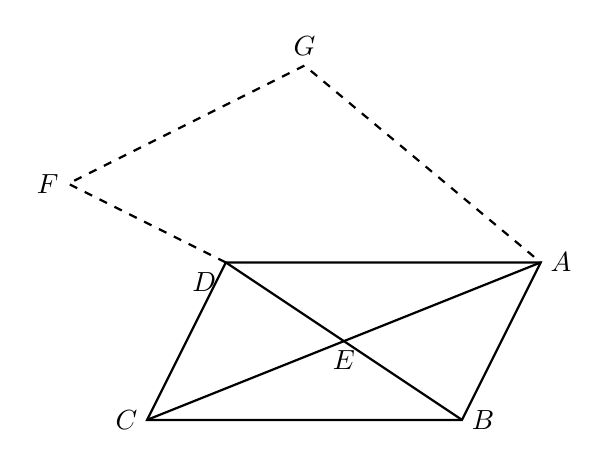
\begin{tikzpicture}[scale=1]
\coordinate (C) at (0,0);
\coordinate (B) at (4,0);
\coordinate (D) at (1,2);
\coordinate (A) at (5,2);
\coordinate (E) at (2.5,1);
\coordinate (F) at (-1,3);
\coordinate (G) at (2,4.5);

\draw[thick] (C) -- (B) -- (A) -- (D) -- cycle;
\draw[thick] (C) -- (A);
\draw[thick] (B) -- (D);
\draw[dashed,thick] (D) -- (F) -- (G) -- (A);

\node[left] at (C) {$C$};
\node[right] at (B) {$B$};
\node[below left] at (D) {$D$};
\node[right] at (A) {$A$};
\node[below] at (E) {$E$};
\node[left] at (F) {$F$};
\node[above] at (G) {$G$};
\end{tikzpicture}
\end{document}
